% !TEX encoding = UTF-8
% !TEX TS-program = pdflatex
% !TEX root = ../tesi.tex
% !TEX spellcheck = it-IT

%**************************************************************
\chapter{Introduzione}
\label{cap:introduzione}
%**************************************************************
xxxx (ignorare fino ad 1.1)\\


\noindent Esempio di utilizzo di un termine nel glossario \\
\gls{api}. \\

\noindent Esempio di citazione in linea \\
\cite{site:agile-manifesto}. \\

\noindent Esempio di citazione nel pie' di pagina \\
citazione\footcite{womak:lean-thinking} \\

%**************************************************************
\section{L'azienda}

VIC è stata fondata da Alessio Bisutti che, dopo aver sviluppato una lunga esperienza nel campo ispettivo, ha deciso di costituire una società in grado di offrire ai propri clienti un servizio professionale, chiaro ed affidabile, appoggiandosi sulle nuove tecnologie.\\
VIC iniziò a Venezia 7 anni fa come piccola società di ispezione locale ed ora il gruppo VIC è uno dei più grandi attori del mercato globale.\\
Fin dall'inizio, l'obiettivo principale di VIC è stata la riduzione del tempo tra ispezione e reporting al cliente. Ora l'obiettivo è raggiunto, perché VIC sta fornendo ai suoi clienti tutti i risultati e le informazioni importanti in tempo reale, senza alcun ritardo, grazie agli investimenti fatti nel campo della tecnologia e delle applicazioni mobile.\\
VIC è la prima ed unica azienda in campo ispettivo ad offrire un'ampia gamma di servizi tecnologici a completa disposizione dei propri clienti. 

%**************************************************************
\section{L'idea}

Mansioni come determinare la corretta forma, peso, quantità e dimensioni degli oggetti da ispezionare sono tra le più importanti per i controlli effettuati dall'azienda.\\
Gli ispettori possono scattare molte fotografie, prendere appunti e sfruttare la loro esperienza per fornire stime accurate; si è manifestata però la necessità di affiancare queste ultime a dei dati quanto più possibile oggettivi e rapidi da ottenere.\\
Da qui nasce l'idea di fornire agli ispettori uno strumento informatico in grado di effettuare queste stime. Grazie alla ricostruzione computerizzata resa disponibile dai \emph{Tango device} sarà possibile non solo visualizzare su uno schermo il modello 3D del soggetto della ispezione, ma anche ottenere ulteriori vantaggi quali:
\begin{itemize}
	\item Avere una stima del volume e quindi del peso della materia prima.
	\item Confrontare l'oggetto con un modello idea, permettendo così un rapido controllo eventuali di danni o deformazioni.
\end{itemize}
Allo stato attuale sono rese disponibili solamente le funzionalità di ricostruzione dell'oggetto e calcolo (approssimato) del volume.\\
Alcune operazioni sarebbero troppo pesanti per le potenzialità del tablet, quindi è stato realizzato un \emph{backend server} per tutte l'elaborazione delle ricostruzioni, mentre la realizzazione delle stesse è affidata all'applicativo per tablet.

\section{Il Prodotto - lato dispositivo}
L'applicazione prodotta risponde, in maniera minimale, alle esigenze citate nel punto precedente.\\
La sua realizzazione presenta molti punti critici e rischi piuttosto difficili da prevedere. Per questo sono stati realizzati molti prototipi, al fine di escludere vie non percorribili e trovare una soluzione soddisfacente.\\
Lo scopo principale della applicazione lato tablet è quello di rilevare ed elaborare un corretto \emph{Point Cloud} dell'oggetto che si vuole ispezionare.\\
Un \emph{Point Cloud} non è altro che una descrizione algebrica di un oggetto tridimensionale ottenuta tramite un insieme, il più possibile fitto, di punti che lo compongono. I dispositivi Tango infatti, grazie al sensore di profondità, cercano di rilevare le triplette di coordinate del maggior numero di punti possibile. Sfruttando questi dati è possibile posizionare dei punti nello spazio in maniera da fornire all'utente una rappresentazione comprensibile dell'oggetto.
\begin{figure}[!h] 
    \centering 
    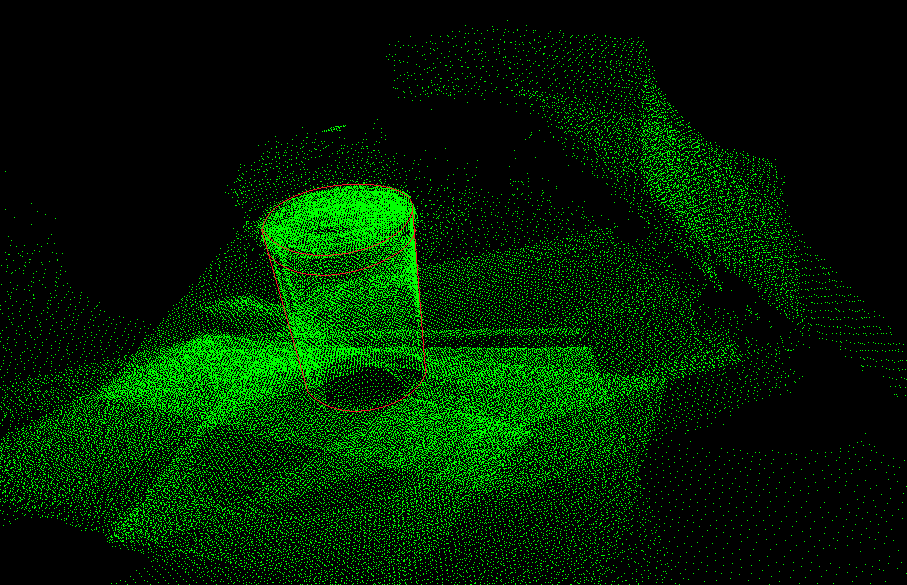
\includegraphics[width=1.0\columnwidth]{pointClouds/bidoneConico.png} 
    \caption{Point Cloud di un bidone Conico}
\end{figure}


\subsection{Primo prototipo}
Il primo prototipo realizzato risponde all'esigenza di catturare e salvare in formato leggibile da un \emph{render} grafico i dati forniti dal sensore di profondità.
Nella sua semplicità ha dato modo allo studente di testare la stabilità delle \emph{API} e produrre della documentazione interna che riportava quali fossero i metodi delle \emph{API} da utilizzare e quali fossero invece quelli poco stabili, sperimentali o addirittura non ancora implementati dal produttore.

\subsection{Secondo prototipo: Cloude}
\subsubsection{Affrontare la discrepanza tra coordinate assolute e coordinate relative}
Un solo \emph{Point Cloud} non è sufficiente a ricostruire un oggetto. Ovviamente il dispositivo, registrando la nuvola di punti inquadrata in un determinato istante, riesce a rilevare solamente i punti che "riesce a vedere": i punti presenti nella parte posteriore dell'oggetto scansionato non possono essere "visti" e conseguentemente nemmeno misurati. Se si vuole avere una ricostruzione completa e non solamente di una facciata è necessario prendere più rilevazioni ed integrarle.\\
Le seguenti immagini mostrano il \emph{Point Cloud} che descrive la parte anteriore di una scatola rettangolare; dato che la ripresa è stata effettuata da di fronte ed in alto solo le facce superiore ed anteriore sono state memorizzate, mentre delle altre non si hanno dati. I contorni sono stati evidenziati successivamente per permettere una migliore comprensione della forma.
\begin{figure}[!h] 
    \centering 
    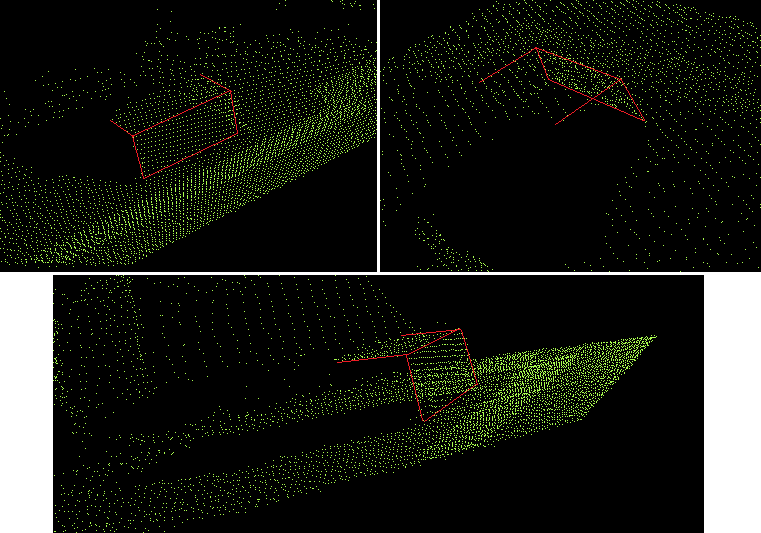
\includegraphics[width=1.0\columnwidth]{pointClouds/singoloShot.png} 
    \caption{Un singolo \emph{Point Cloud}}
\end{figure}
\subsubsection{Approccio}
Questo prototipo, denominato \emph{Cloude}, è stato realizzato allo scopo di rispondere a questa esigenza. L'idea che ne sta a fondamento è la seguente:
\begin{itemize}
	\item Permettere all'utente di scattare alcune foto all'oggetto, quindi di rilevare diversi \emph{Point Cloud}.
	\item Tenere costantemente traccia della posizione del dispositivo, in particolare delle posizioni nei momenti in cui vengono scattate le foto.
	\item Usare la posizione relativa al \emph{Point Cloud} per traslare e ruotare lo stesso punto a punto, riducendo così le coordinate a dei valori assoluti.
	\item Ora le nuvole di punti registrate sono sovrapponibili le une con le altre e forniscono una prima ricostruzione dell'oggetto.
\end{itemize}

\subsection{Terzo prototipo: Samba}
Il prototipo precedente generava delle ricostruzioni riconoscibili, ma piuttosto imprecise.\\
Una analisi dello stesso ha fatto emergere diverse criticità che sono state documentate, assieme alle possibili soluzioni, all'interno di un documento descrittivo. Quest'ultimo è stato alla base dello sviluppo di \emph{Samba}.
\subsubsection{Eccessiva complessità dell'elaborazione}
\emph{Cloude} sfrutta un metodo delle librerie \emph{Tango} che trasforma le coordinate di un singolo punto in coordinate assolute fruttando la posizione relativa a cui si trovava il dispositivo, permette di scrivere poco codice, ma ha una elevata complessità. Ciò comporta un sensibile rallentamento dell'elaborazione dei \emph{Point Cloud}. Un \emph{cloud} medio conta intorno ai 90000 punti e con questo approccio richiede mediamente 1,5-2 secondi per essere completamente elaborato, tempo non accettabile per lo scopo per cui l'applicazione è pensata.\\
In \emph{Samba} è stato cambiato radicalmente approccio:
\begin{itemize}
	\item Ad ogni \emph{Point Cloud} viene associata una matrice di trasformazione e non la posizione stessa.
	\item In questo modo è sufficiente moltiplicare ogni punto (vettore) per la matrice, che viene calcolata una sola volta per ogni \emph{Point Cloud}. 
	\item Si è ottenuta così una complessità di \texttt{O(n)} sul numero dei punti da trasformare riducendo i tempi di elaborazione da 1,5-2s a circa 200ms (sullo stesso dispositivo).
\end{itemize}
\subsubsection{Bassa qualità delle ricostruzioni}
Nelle ricostruzioni generate da \emph{Cloude} gli oggetti appaiono deformati, spesso i vari \emph{Point Cloud} non si sovrappongono correttamente generando fenomeni di \emph{ghosting}, talvolta rendendo addirittura irriconoscibile l'oggetto.\\
Questo è dovuto ad una scorretta stima della posizione del dispositivo, che induce il calcolo di una erronea matrice di trasformazione, e quindi ad un errato posizionamento delle nuvole di punti all'interno dello spazio.\\
Il fenomeno in questione è detto \emph{"drifting"}: i \emph{device Tango}, esattamente come le più comuni applicazioni in realtà aumentata, utilizzano la tecnica del \emph{Motion Tracking} che consiste nel calcolare la propria posizione frequentemente ed in maniera relativa alla coordinate acquisite nella stima precedente. Per quando queste stime siano estremamente precise generano una catena di piccoli errori che sommati tra loro molto presto portano ad una importante discrepanza tra la posizione stimata dal dispositivo e quella reale. Ad esempio partendo da una determinata posizione e camminando in cerchio è praticamente impossibile che la traiettoria stimata passi nuovamente per il punto di partenza.
\begin{figure}[!h] 
    \centering 
    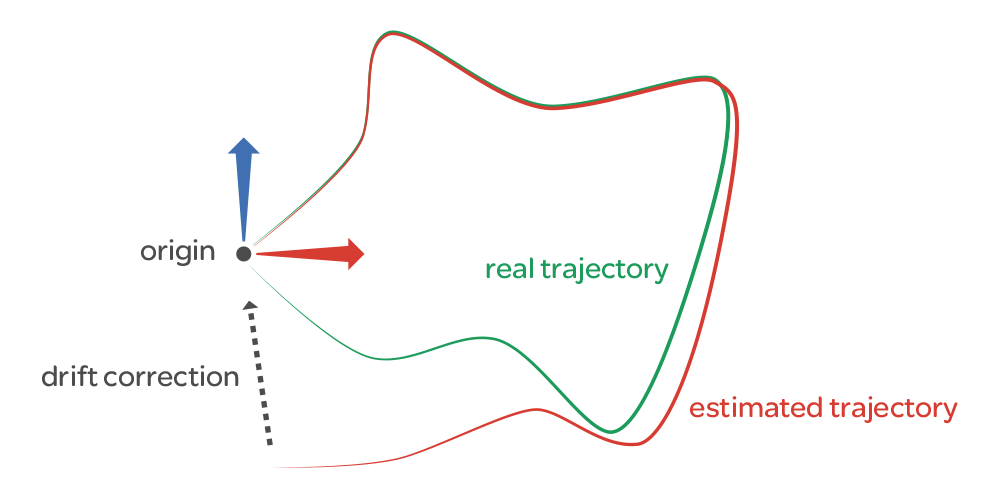
\includegraphics[width=0.9\columnwidth]{varie/Drift_Correction.png} 
    \caption{Motion Tracking}
\end{figure}
Ciò è un limite fisico dei dispositivi, ed è nella pratica impossibile da eliminare, in quanto sarebbe necessario azzerare completamente gli errori relativi.\\
La tecnologia \emph{Tango} però fornisce un altro meccanismo di localizzazione: l'\emph{Area Learning}. Le applicazioni ideate per questo tipo di dispositivi infatti hanno la possibilità di mantenere memoria degli spazi che visitano, e successivamente usare queste informazioni per localizzarsi.\\
Il meccanismo è piuttosto simile a quello della memoria spaziale umana: una persona portata bendata all'interno di un edificio sconosciuto, una volta liberata, non avrà alcun mezzo per intuire dove si trovi; se invece la stessa persona fosse condotta all'interno della propria abitazione, alla prima sbirciata noterebbe immediatamente qualche particolare che gli farebbe immediatamente recuperare l'orientamento.\\
Allo stesso modo il tablet è in grado memorizzare alcune \emph{features} all'interno dell'ambiente ed usarle come faro per la triangolazione. \\
Memorizzare completamente un ambiente tuttavia è una operazione che richiede parecchio tempo e costringe l'utente a muoversi per diversi minuti inquadrando tutti i dettagli del luogo dove si trova. Per rendere l'applicazione maggiormente responsiva e più vicina alle esigenze dell'utenza \emph{Samba} adotta un approccio detto \emph{Drift Correction}: inizialmente è richiesto all'utente di inquadrare per una ventina di secondi l'ambiente, in maniera da permettere la creazione di una minimale memorizzazione, successivamente il \emph{Motion Tracking} è usato per piccoli spostamenti ma viene corretto non appena venga inquadrata qualcuna delle (poche) \emph{features} memorizzate. Trasparentemente all'utente, in background, il processo di \emph{Area Learning} continua, memorizzando sempre nuovi dettagli e conseguentemente aumentando sempre più la qualità della registrazione.\\

\subsubsection{Dimensioni eccessive dei file, ridondanza dei punti sovrapposti}
Data la grande mole di punti registrati dai sensori di profondità i \emph{file} contenenti le ricostruzioni generati da \emph{Cloude} sono di dimensione eccessiva, anche più di 10Mb una decina scatti.
Considerando che idealmente gli scatti da riprendere potrebbero essere molti e spesso dovranno essere inviati al \emph{Server} tramite connessione a consumo il peso di questi \emph{file} non è da trascurare.\\
Inoltre c'è una grossa ridondanza di punti: è comune caso d'uso che una stessa zona venga inquadrata in più scatti, quindi tali \emph{Point Cloud} ruotati ed uniti presenterebbero molti punti con le stesse coordinate e semplicemente sovrapposti, quindi senza dare alcuna informazione aggiuntiva.\\
\emph{Samba} risolve questo problema utilizzando un leggero \emph{voxeling}, ovvero suddividendo lo spazio in cubi o \emph{voxel} di lato prefissato e registrando quali sono i \emph{voxel} che contengono i punti della nuvola.
Scegliendo una opportuna definizione, ovvero una opportuna dimensione dei \emph{voxel}, si può ottenere una ricostruzione comunque con un buon livello di dettaglio, ma priva di ridondanza dei punti e quindi meno pesante in termini di memoria.\\
Dopo diversi test è emerso che definizioni più fine di 10 millimetri non portano a nessun effettivo miglioramento della qualità della ripresa, e quindi questo è stato scelto come definizione predefinita.
\begin{figure}[!h] 
    \centering 
    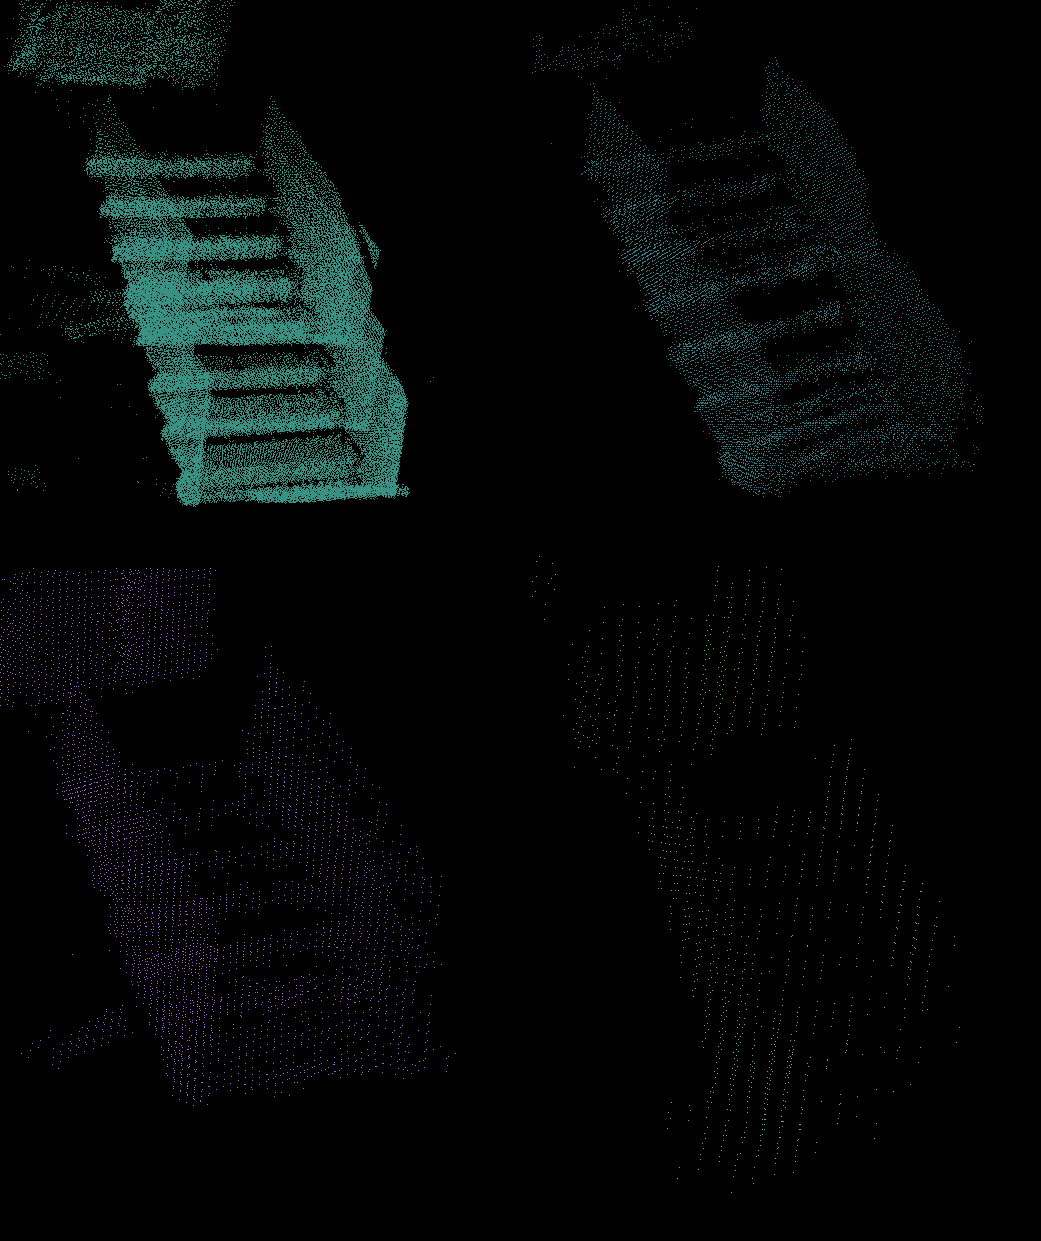
\includegraphics[width=0.9\columnwidth]{pointClouds/voxeling.png} 
    \caption{Rappresentazione tramite \emph{Point Cloud} della stessa scalinata usando \emph{voxeling} a 10, 25, 50, 100 millimetri.}
\end{figure}

\subsection{Ulteriore incremento di Samba, il prototipo finale}
\emph{Samba}, nella sua prima realizzazione, soddisfaceva completamente gli obiettivi fissati per quanto riguarda la \emph{business logic} tuttavia è risultato carente nell'interfacciarsi con l'utente.\\
Quindi è stato pianificato un ulteriore ciclo di raffinamento che ha portato questo prototipo allo stato attuale. Segue una breve lista delle principali migliorie.

\subsubsection{Preview dell'inquadratura}
\label{cap:frame_preview}
La sola preview della fotocamera a colori si è rivelata non sufficiente. Oltre a non fornire una chiara idea dei punti che verranno registrati non da la possibilità all'utente di controllare se la foto che sta per scattare sia "buona" oppure no.\\
Il sensore di profondità sfrutta la tecnologia \emph{infrared} e per questo è soggetto a tutti i limiti fisici di quest'ultima; sono emerse, infatti, grosse difficoltà nel misurare i punti
\begin{itemize}
	\item di una superficie molto scura.
	\item di una superficie riflettente o particolarmente lucida.
	\item all'interno di stanze con illuminazione scarsa o assente.
\end{itemize}
A volte il problema è insormontabile e la ricostruzione non potrà avvenire con successo, altre è sufficiente trovare una buona posizione per permettere al sensore di effettuare le misurazioni. Questo rende necessario mostrare sullo schermo non solo quello che "vede" la fotocamera, ma anche quello che "vede" il dispositivo \emph{infrared}.\\
A questo scopo è stata parzialmente riusata una applicazione di prova fornita sotto licenza \emph{Open Source} dalla \emph{Google}\footcite{GitHub: https://github.com/googlesamples/tango-examples-java} e che utilizza la libreria grafica \emph{Rajawali}\footcite{GitHub: https://github.com/Rajawali/Rajawali}.\\
Il \emph{render} in questione è moto semplice ma efficace ed aumenta il valore aggiunto dell'applicazione dandole un aspetto gradevole e permettendo all'utente di avere aggiornamenti in tempo reale sul \emph{Point Cloud} inquadrato.
\begin{figure}[!h] 
    \centering 
    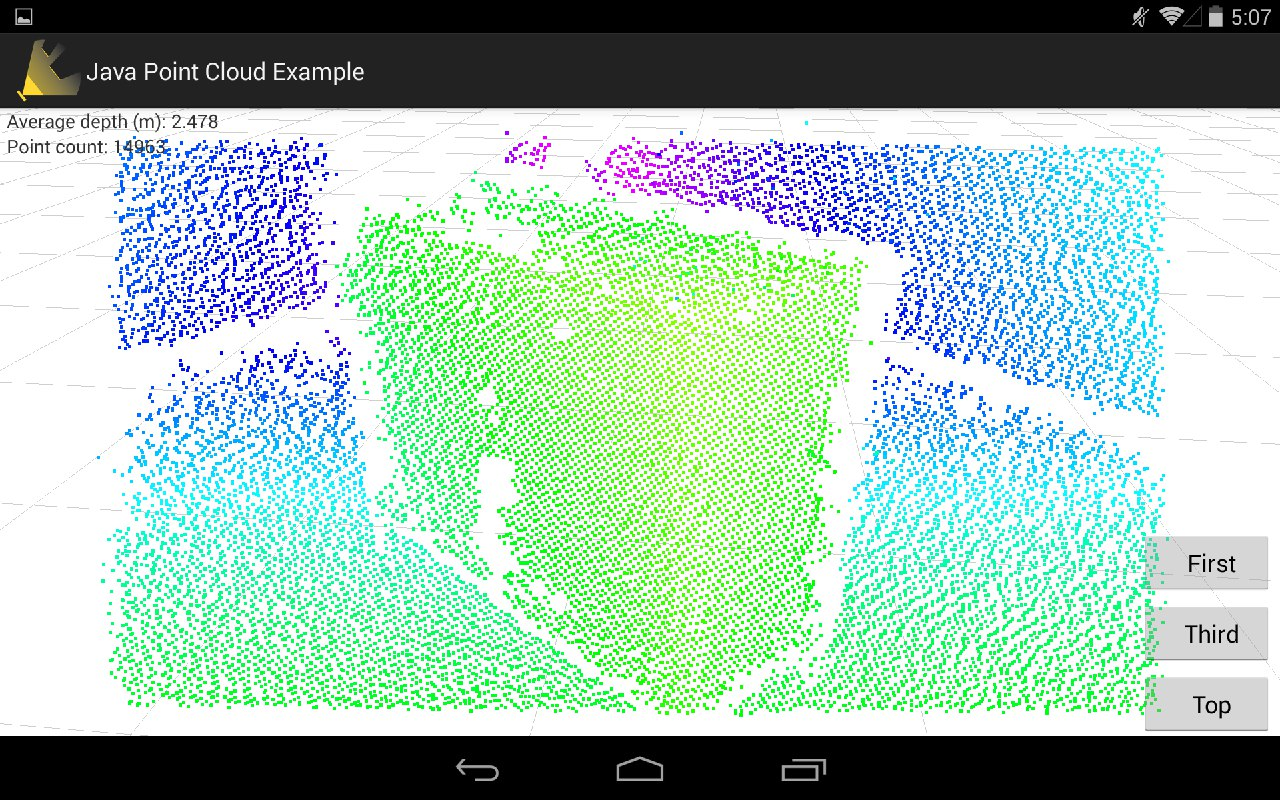
\includegraphics[width=1.0\columnwidth]{varie/rajawaliRenderer.jpg} 
    \caption{Il render di Java Point Cloud Example mentre viene inquadrata una cassettiera}
\end{figure}


\subsubsection{Visualizzazione su tablet del \emph{Point Cloud} ricostruito}
Con il \emph{render} descritto nel punto precedente è possibile visualizzare ciò che "vede" il sensore di profondità in tempo reale. Questo tuttavia non è sufficiente: mano a mano che si effettua la ripresa, in background viene calcolata la ricostruzione dell'oggetto in analisi, non poterlo visualizzare sul \emph{tablet}, ma solo lato \emph{server} appare quantomeno frustrante e soprattutto non da la possibilità all'utente di avere una idea dello stato in cui è la ricostruzione. \\
Per questo si è pensato di sfruttare lo stesso meccanismo di \emph{rendering} per far visualizzare all'utente la ricostruzione che sta effettuando. É quindi stata aggiunta la possibilità di alternare tra la visualizzazione in tempo reale e la visualizzazione dell'intera ricostruzione generata.\\
\begin{figure}[!h] 
    \centering 
    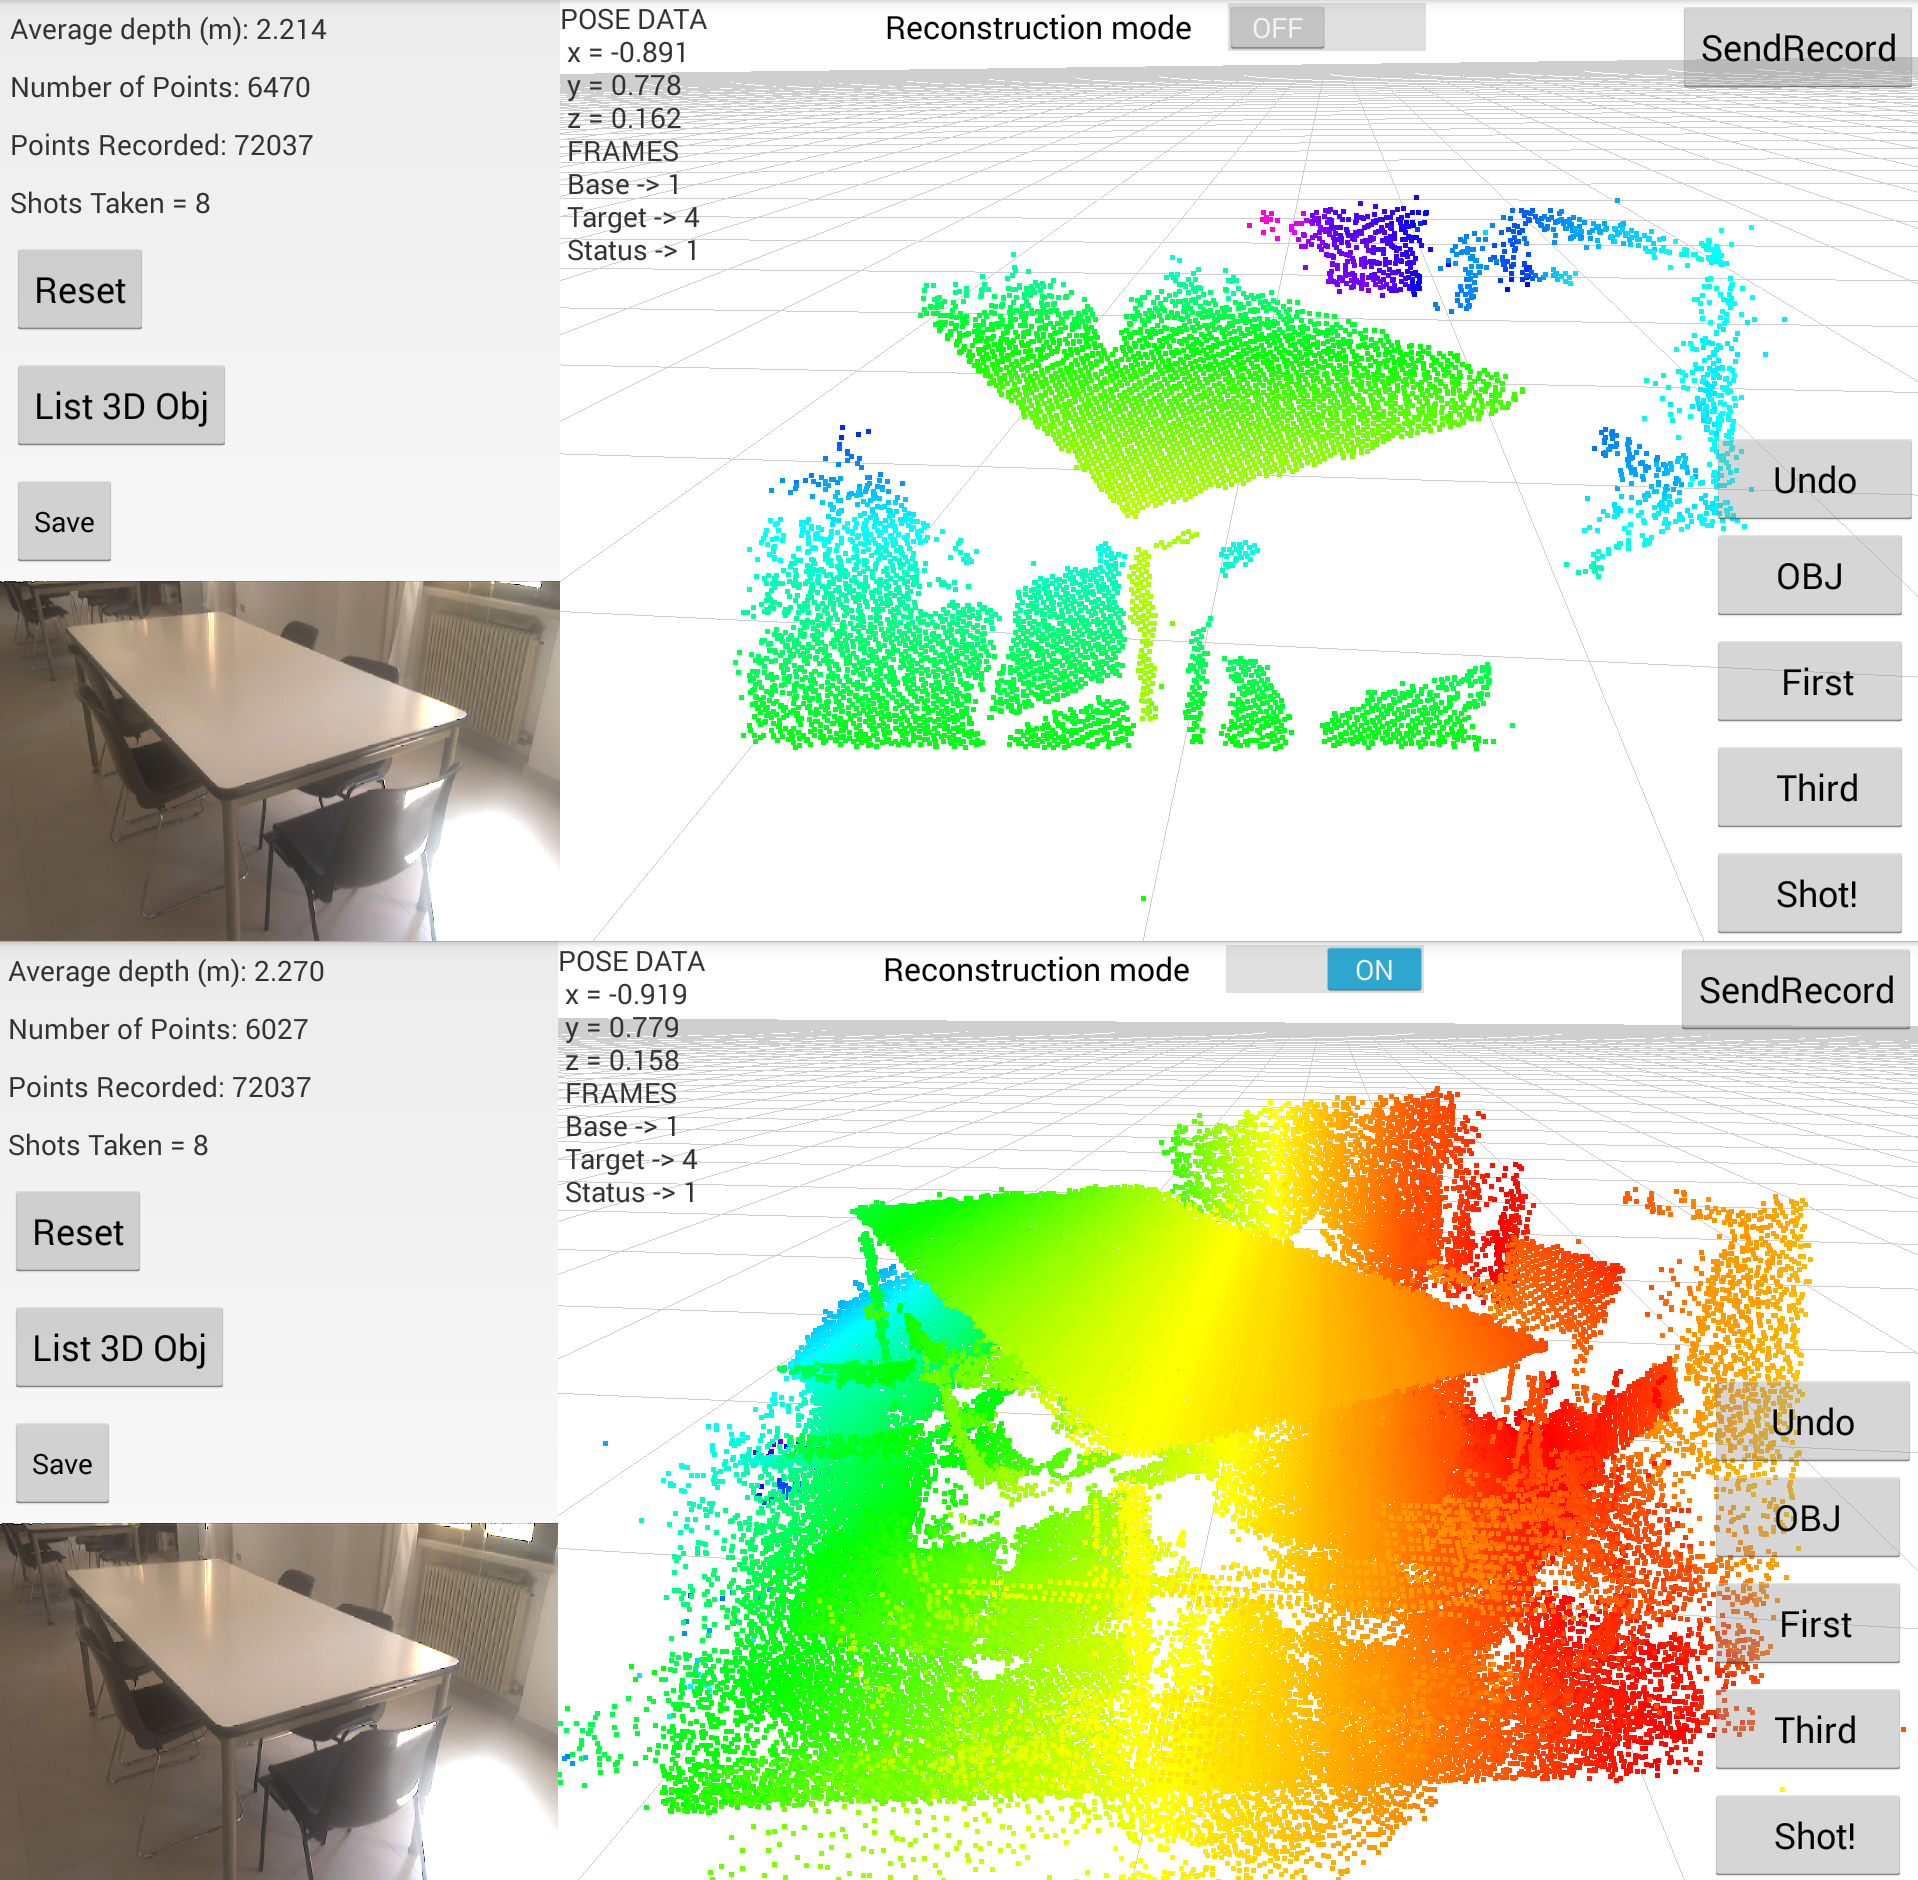
\includegraphics[width=1.0\columnwidth]{varie/sambaRenderer.png} 
    \caption{Le due modalità del render di \emph{Samba}: in alto la visualizzazione in tempo reale, in basso la visualizzazione della ricostruzione.}
\end{figure}


\subsubsection{Aggiunta operazioni di undo}
Nonostante gli sforzi per mantenere una alta qualità delle riprese qualcuno dei \emph{Point Cloud} catturati continua a presentare grossi difetti (come errato posizionamento, deformità, grossa presenza di rumore etc).
Importante miglioria effettuata in questa fase è stata l'inserimento della possibilità di annullare un certo numero di operazioni; in questo modo le riprese che contengono dei difetti possono essere scartate e ripetute.

\subsubsection{Istruzioni per l'utente}
Questa applicazione, come tutte le applicazioni \emph{Tango}, introduce nuove azioni che l'utente deve compiere per mettere il dispositivo nella condizione di poter operare al meglio; ed è compito degli applicativi istruire l'utente sul comportamento da tenere.\\
Ad esempio, durante l'avvio dell'\emph{app}, l'utente deve avere cura di mantenere il \emph{tablet} in posizione verticale ed il più possibile fermo. Questa, come la maggior parte delle indicazioni, possono essere notificate all'utente tramite un \emph{framework} messo a disposizione dal produttore in grado di integrare segnali e notifiche all'interno del ciclo di vita dell'applicazione stessa.\\
Fanno eccezione le istruzioni che devono essere date all'utente durante la fase di localizzazione. Le \emph{API Tango} non forniscono alcun aiuto per stabilire se il dispositivo si sia orientato o meno. È stato quindi necessario studiare delle euristiche capaci di intuire se il dispositivo "si senta o meno a proprio agio".\\
L'idea sta nello sfruttare il fatto che i dispositivi \emph{Tango}, una volta imparato un ambiente, fissano l'origine $O$ del loro sistema di riferimento (per quel particolare ambiente) in un punto arbitrario dello stesso. Alla luce di questo è sufficiente richiedere, durante la fase di localizzazione, la posizione della suddetta origine rispetto ad un punto speciale detto \emph{start-of-service point} che chiameremo $S$, ovvero il punto in cui era il dispositivo al momento dell'avvio dell'applicazione.\\
\begin{figure}[!h] 
    \centering 
    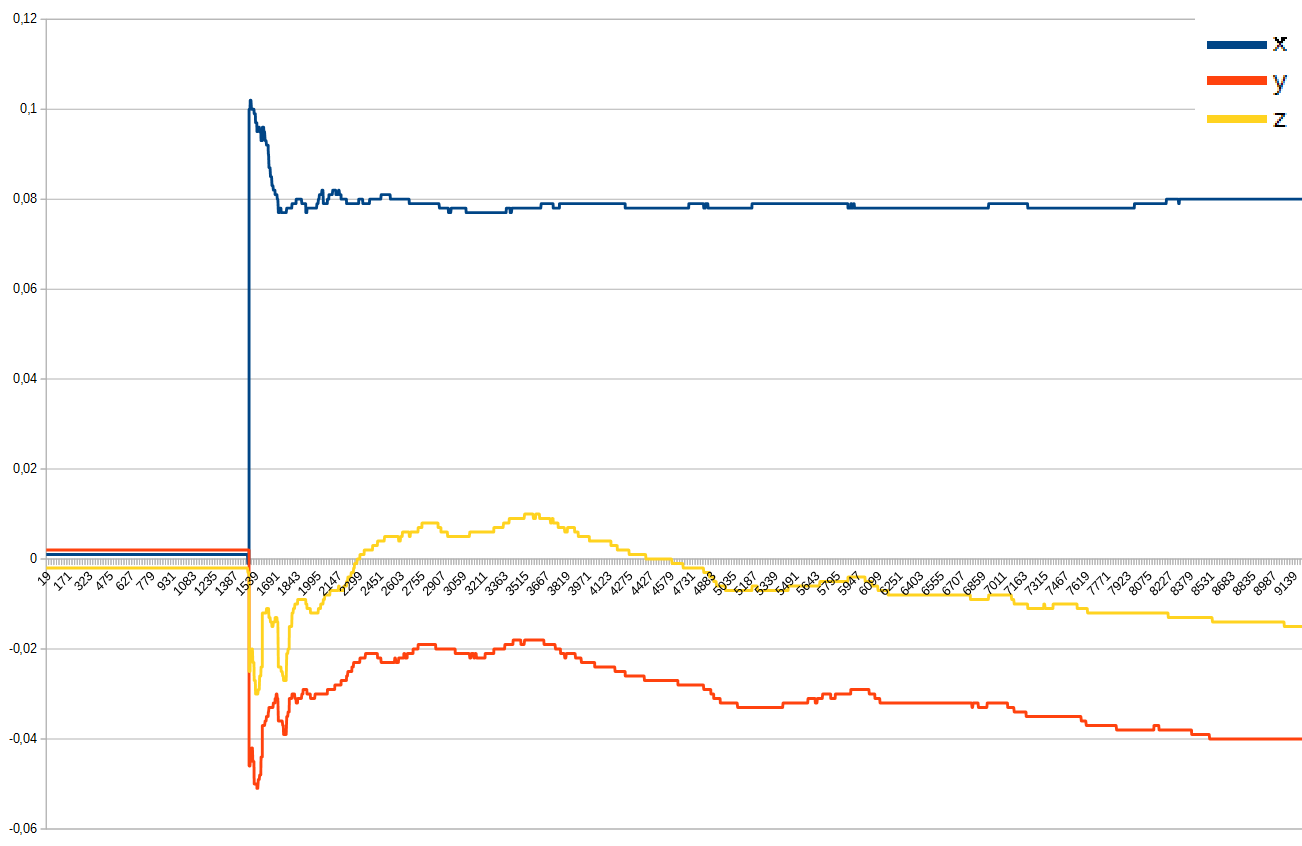
\includegraphics[width=1.0\columnwidth]{grafici/fluttuazioneCoordDriftCorrection.png} 
    \caption{Grafico della coordinate di $S$ rispetto ad $O$ durante la fase di inizializzazione della \emph{Drift Correction}}
\end{figure}
\\
Il grafico in figura rappresenta le coordinate $x$, $y$ e $z$ della distanza con segno tra $O$ ed $S$ nel primo minuto circa di attività dell'applicazione. Esso può essere diviso in tre fasi:
\begin{itemize}
	\item Inizialmente la distanza molto è vicina a zero. Prima che avvenga la localizzazione il sistema \emph{Tango} non ha altra scelta che posizionare $O$ nelle stesse coordinate di $S$.
	\item Successivamente avverrà un brusco cambiamento nella distanza tra questi due punti perché tutto d'un tratto il sistema riconoscerà qualche \emph{feature} e sposterà immediatamente l'origine degli assi. Questa fase non è  ancora stabile in quanto l'ambiente è ancora in fase di riconoscimento e l'origine $O$ verrà traslata spesso.
	\item Una volta riconosciuto correttamente l'ambiente (nella seconda metà del grafico) si può notare che tutte le coordinate si stabilizzano ad una distanza quasi fissa. Da questo momento in avanti si avrà una buona localizzazione e l'utente potrà iniziare la rilevazione.
\end{itemize}
La distanza tra $O$ ed $S$ dovrebbe essere idealmente costante. Si è notato sperimentalmente, però, che non è così: a causa di limiti fisici del dispositivo essa continuerà a fluttuare entro un paio di centimetri di raggio. Ciò a volte può creare qualche piccolo errore nella ricostruzione, ma per oggetti piuttosto grandi esso è trascurabile.


\section{Il Prodotto - lato server}
L'applicazione lato server si occupa di "pulire" la ricostruzione dagli elementi inutili, come ad esempio pavimento, rumore, oggetti di sfondo e convertirla in un formato portabile.\\
\subsection{Point Cloud Library}
\emph{PCL} o \emph{Point Cloud Library} è una libreria \emph{Open Source} e \emph{Large Scale} per l'elaborazione di 2D e 3D di immagini e \emph{Point Cloud}. Fornisce diversi filtri ed algoritmi in grado di risolvere molti dei problemi che sono stati riscontrati per quando riguarda l'elaborazione delle ricostruzioni.\\
L'applicativo lato server fa vasto uso di questa libreria.
\subsection{Generazione mesh}
Per poter elaborare facilmente la ricostruzione ed ottenere un modello portabile è necessario trasformare la nuvola di punti in una \emph{mesh}, ovvero una rappresentazione di un oggetto 3D che consiste in un insieme di facce poligonali, solitamente semplici triangoli. Inoltre tutti i più diffusi formati per oggetti tridimensionali come \texttt{obj} e \texttt{ply} sono in grado di rappresentare solamente \emph{mesh}.\\
Per ottenere una buona riproduzione dell'oggetto l'applicativo applica diversi filtri:
\begin{itemize}
	\item \textbf{sparse filter / filter radius}: vengono eliminati i punti isolati ed i punti ad una eccessiva distanza dal centro, i quali sono quasi sempre frutto di errori nelle misurazioni.
	\item \textbf{filter ground}: viene eliminato il pavimento.
	\item \textbf{voxel filter}: viene effettuata una ulteriore operazione di voxeling allo scopo di ridurre la mole di calcoli e regolarizzare il \emph{Point Cloud}.
	\item \textbf{cluster extractor}: si cerca di suddividere la ricostruzione nei vari oggetti da cui è composta, dopodiché si mantiene solamente l'oggetto (o \emph{cluster}) che si trova più al centro.
	\item \textbf{meshing}: i punti rimanenti sono solamente quelli dell'oggetto in analisi. Essi vengono usati per generare la \emph{mesh}.
\end{itemize}
Al termine di questo processo si ottiene l'oggetto 3D, che può essere convertito nel formato preferito. L'immagine sottostante mostra il processo di elaborazione dell'immagine di una scatola rettangolare. Si possono osservare, da in alto a sinistra ad in basso a destra: la ricostruzione fornita dal \emph{tablet}, il \emph{Point Cloud} risultante da \emph{sparseFilter} e \emph{filterRadius}, l'output della operazione di rimozione del pavimento, il risultato del \emph{voxelFilter}, il \emph{cluster} estratto ed infine la \emph{mesh} dell'oggetto.
\begin{figure}[!h] 
    \centering 
    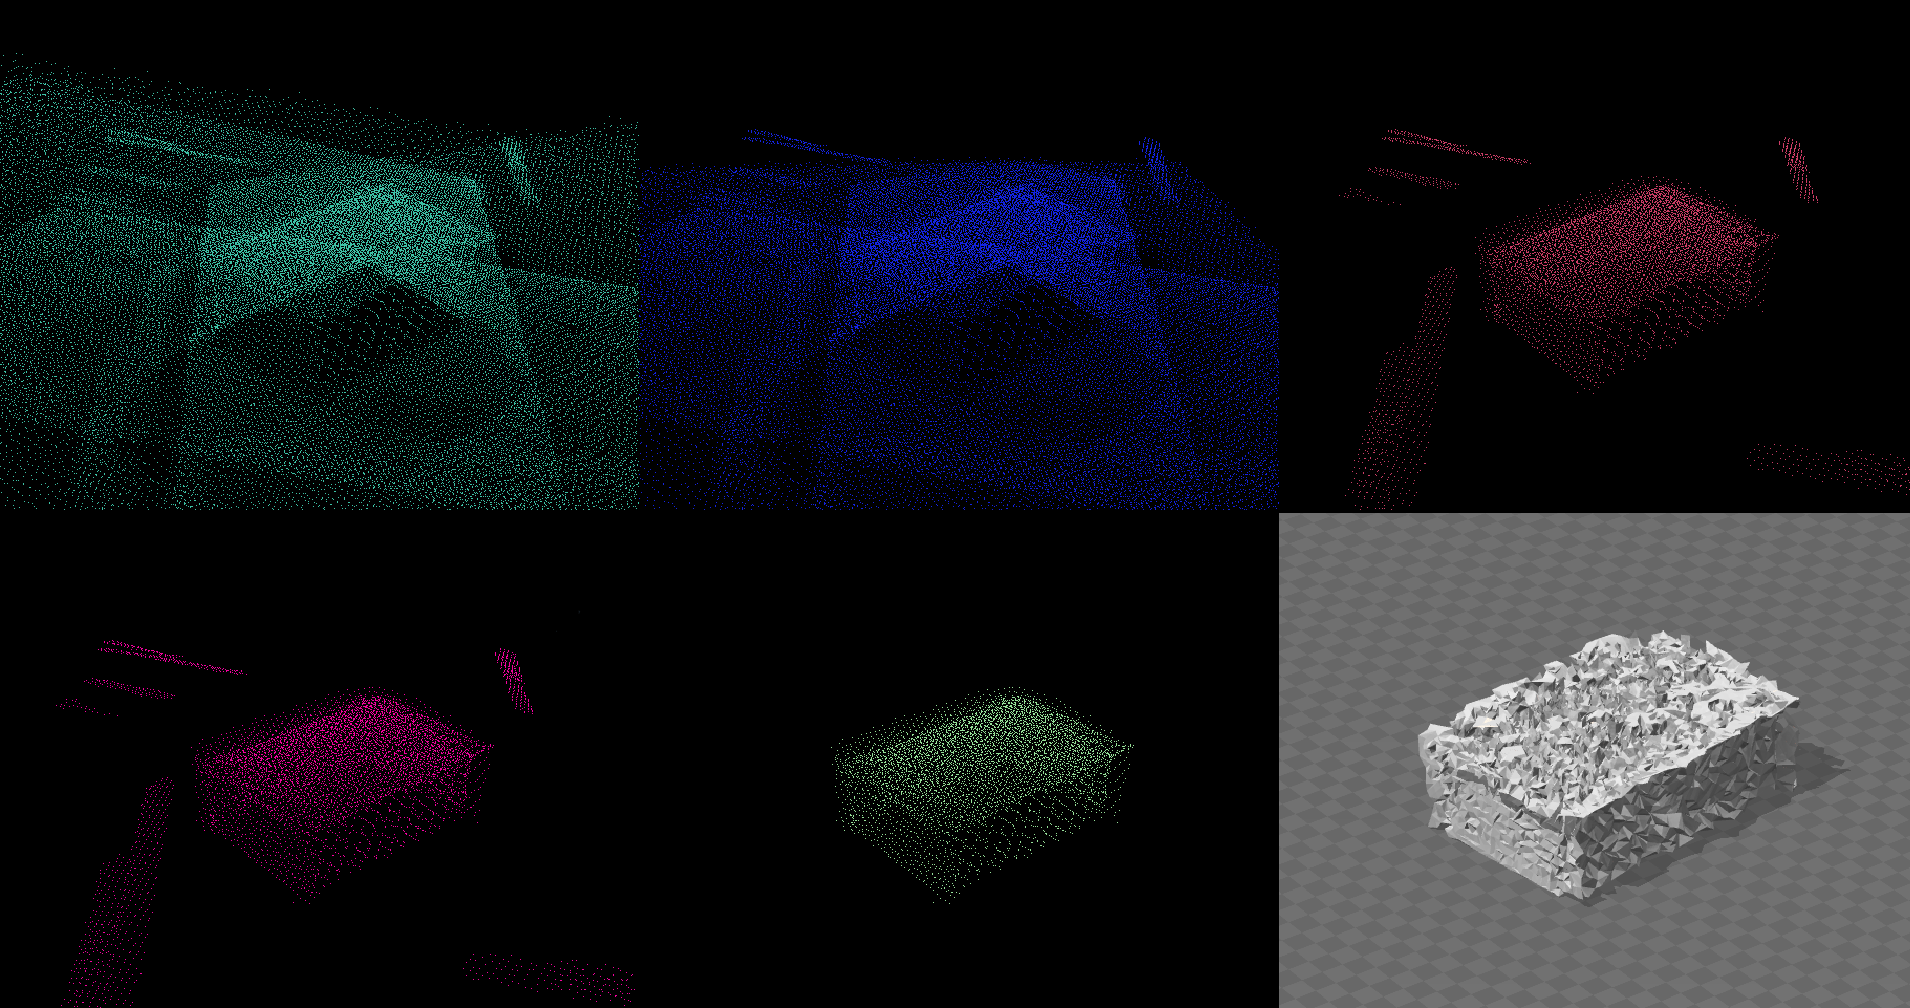
\includegraphics[width=1.2\columnwidth]{pointClouds/processoMesh.png} 
    \caption{Input ed Output del processo di meshing}
\end{figure}

\subsection{Calcolo del volume}
Una volta ottenuta la \emph{mesh} il calcolo del volume è piuttosto immediato. A questo fine è stato sfruttato il risultato di una pubblicazione di \emph{Cha Zhang} e \emph{Tsuhan Chen} dal titolo \emph{EFFICIENT FEATURE EXTRACTION FOR 2D/3D OBJECTS
IN MESH REPRESENTATION}\footcite{site: http://research.microsoft.com/en-us/um/people/chazhang/publications/icip01_ChaZhang.pdf}.
Il trucco è calcolare, per ogni triangolo che compone la \emph{mesh}, il volume con segno del tetraedro che ha il triangolo stesso come base e il quarto vertice in un punto fissato, scelto internamente alla \emph{mesh}, per evitare eventuali problemi di instabilità numerica. Il segno del volume è dato dalla direzione della normale al piano del triangolo. Questi volumi, sommati tra loro, restituiscono il volume convesso della \emph{mesh}.


%**************************************************************
\section{Organizzazione del testo}
xxxx
%\begin{description}
%
%    \item[{\hyperref[cap:processi-metodologie]{Il secondo capitolo}}] descrive ...
%    
%    \item[{\hyperref[cap:descrizione-stage]{Il terzo capitolo}}] approfondisce ...
%    
%    \item[{\hyperref[cap:analisi-requisiti]{Il quarto capitolo}}] approfondisce ...
%    
%    \item[{\hyperref[cap:progettazione-codifica]{Il quinto capitolo}}] approfondisce ...
%    
%    \item[{\hyperref[cap:verifica-validazione]{Il sesto capitolo}}] approfondisce ...
%    
%    \item[{\hyperref[cap:conclusioni]{Nel settimo capitolo}}] descrive ...
%\end{description}

Riguardo la stesura del testo, relativamente al documento sono state adottate le seguenti convenzioni tipografiche:
\begin{itemize}
	\item gli acronimi, le abbreviazioni e i termini ambigui o di uso non comune menzionati vengono definiti nel glossario, situato alla fine del presente documento;
	\item per la prima occorrenza dei termini riportati nel glossario viene utilizzata la seguente nomenclatura: \emph{parola}\glsfirstoccur;
	\item i termini in lingua straniera o facenti parti del gergo tecnico sono evidenziati con il carattere \emph{corsivo}.
\end{itemize}